% !TeX root = ../bbchallenge-paper.tex

\newpage

\begin{figure}[h!]
    \centering
    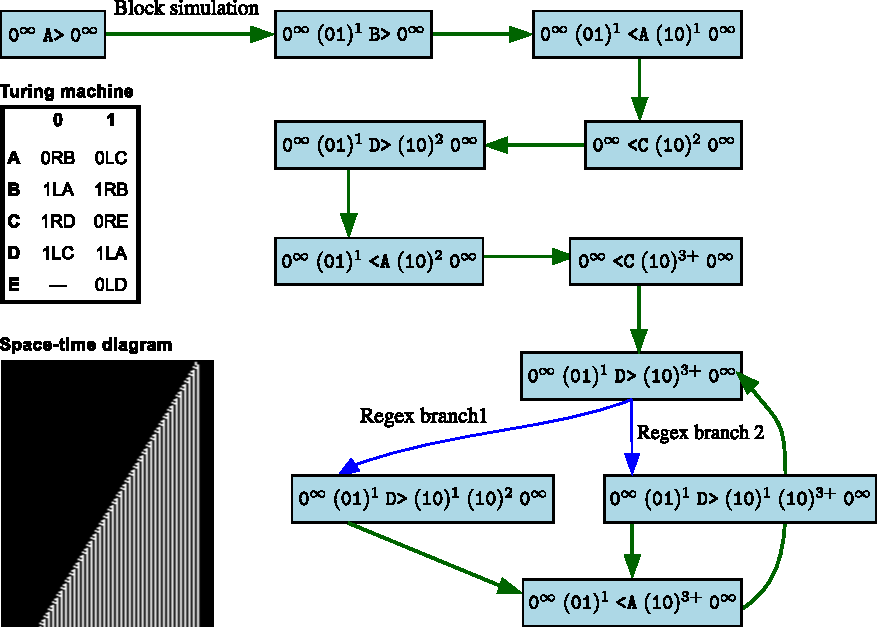
\includegraphics[scale=0.8]{figures/RepWL/RepWL_graph.pdf}
    \caption{{\small Closed graph of regex configurations constructed by the Repeated Word List (RepWL) method for machine \url{https://bbchallenge.org/0RB0LC_1LA1RB_1RD0RE_1LC1LA_---0LD} with block size $l=2$ and block repeat threshold $T=3$. As illustrated by its 300-step space-time diagram, the machine is a simple Translated Cycler which can be easily handled by Section~\ref{alg:loops}, but it has the advantage of having a very small RepWL graph, suitable as an introductory example for the method. Because the graph is closed and contains not halting configuration, the machine does not halt, Theorem~\ref{th:repwl}.}}\label{fig:repWL}
\end{figure}

\subsection{Repeated Word List (RepWL)}\label{sec:RepWL}

The Repeated Word List (RepWL) technique is based on the following simple idea: if a word (or \textit{block}) of length $l > 0$ appears consecutively on the tape more than $T > 0$ times (with $l, T \in \mathbb{N}$ fixed) then, we assume it may repeat an unbounded number of times in the future. In practice, it means we represent configurations as regular expressions. For instance, consider the following configuration:

$$ \texttt{0}^\infty \; \texttt{11100 A> 11110101010111111111} \; \texttt{0}^\infty$$

Using $l=2$ and $T = 3$, we represent it as:

$$ \texttt{0}^\infty \; (\texttt{01}) \; (\texttt{11}) \; (\texttt{00}) \; \texttt{A>} \; (\texttt{11})^2 \; (\texttt{01})^{3+} \; (\texttt{11})^{3+} \; \texttt{0}^\infty $$

Where blocks are constructed from the head outwards, and pumping symbols \szero out of $0^\infty$ if the number of symbols on either part of the tape is not a multiple of $l$. Any repetition of more than $T$ times the same word $w \in \{\szero,\sone\}^l$ is replaced by the regular expression $(w)^{T+}$ meaning that word $w$ is repeated at least $T$ times, hence the only exponents to ever be used in this representation are $\{1,2,\dots,T-1\}$ and $T+$. Note that here, we use \textit{directional head notation} for Turing machines, where the head lives in between cells and points either right or left. This framework is equivalent to the Turing machines setup (Appendix~\ref{app:TMs}) used elsewhere in this work.

Using the rules explained below (\textit{block simulation} and \textit{regex branching}), {\sc decider-RepWL} (Algorithm~\ref{alg:RepWL}) simulates Turing machines directly on these regex configurations starting from the initial configuration (\ie $\texttt{A>}$), as to create a graph of such regex configurations to explore. If this graph is eventually closed (Algorithm~\ref{alg:RepWL}~l.\ref{alg:RepWL:closed}) and contains no halting configuration then we know that the machine will never halt (Theorem~\ref{th:repwl}) since we have constructed a set of configurations bigger than the one it will visit and that does not contain any halting transition. Because there is no guarantee the graph is closed, we also need an additional gas parameter (named $N$ in Algorithm~\ref{alg:RepWL}) indicating how many distinct nodes we're willing to visit at most.

For simulating Turing machines on regex configurations we need to deal with two cases: (i) \textit{block simulation} when the head is facing a constant block (\ie block without a $+$), such as $\texttt{A>} \; (\texttt{11})^2$ and (ii) \textit{regex branching} when the head is facing a block with a $+$, \eg $\texttt{B>} \; (\texttt{01})^{3+}$.

\paragraph{Block simulation.} When the head is facing a constant block, such as in the above example $\texttt{A>} \; (\texttt{11})^2$ (or if the head is at the tape's extremity, we add constant block $(\szero^l)^1$), we can proceed to \textit{block simulation} (also referred to as performing a \textit{macro step}).
Block simulation consists of simulating the Turing machine until the head eventually leaves the block or until a maximum step limit is reached (parameter named $B$ in Algorithm~\ref{alg:RepWL}). Note that the TM may never leave the block if it enters an infinite cycle which is why we need the step limit -- one could alternatively implement cycle detection (Section~\ref{sec:loops}) in block simulation but it is not the route taken in \CoqBB. Depending upon which Turing machine is being simulated, block simulation from block simulation from $\texttt{A>} \; (\texttt{11})^2$ could produce, for instance, $(\texttt{00})^2 \; \texttt{B>}$ or $\texttt{<C} \; \texttt{10} \; \texttt{11} $ or enter a cycle and never leave the block. After block simulation, identical contiguous blocks are regrouped into powers, \eg $(\texttt{10})^1 \; (\texttt{10})^1 \; \texttt{B>}$ becomes $(\texttt{10})^2 \; \texttt{B>}$ and, assuming $T=3$, $(\texttt{10})^2\; (\texttt{10})^1\; \texttt{B>}$ would become $(\texttt{10})^{3+}\; \texttt{B>}$.

\paragraph{Regex branching.} When the head is facing a block with a $+$, for instance $\texttt{B>} \; (\texttt{01})^{3+}$, we add two configurations to the set of configurations to visit next:
\begin{enumerate}
    \item A configuration where $\texttt{B>} \; (\texttt{01})^{3+}$ is replaced with $\texttt{B>} \; (\texttt{01}) \; (\texttt{01})^{2}$
    \item A configuration where $\texttt{B>} \; (\texttt{01})^{3+}$ is replaced with  $\texttt{B>} \; (\texttt{01}) \; (\texttt{01})^{3+}$
\end{enumerate}
In both case, we've reduced to block simulation.

\begin{example}
    Figure~\ref{fig:repWL} gives the RepWL graph for machine \url{https://bbchallenge.org/0RB0LC_1LA1RB_1RD0RE_1LC1LA_---0LD}. This machine was chosen for its very small RepWL graph but it has a very simple behavior (translated cycler, see Section~\ref{sec:loops}).
\end{example}

\ \\
Finally, {\sc decider-RepWL} is correct:

\begin{theorem}[\CoqBB: \texttt{Lemma RepWL\_ES\_decider\_spec}]\label{th:repwl}
    Let $\mathcal{M}$ be a Turing machine $l\in \N^+$ the block-length parameter, $T \in \N^+$ the block repeat threshold, $B \in \N$ the maximum number of steps allowed in block simulation and $N \in \N$ the maximum number of nodes we are willing to visit. Then, \textsc{decider-RepWL}($\mathcal{M}$, $l$, $T$, $B$, $N$) terminates and its result is correct -- see Algorithm~\ref{alg:RepWL}: if it returns \NONHALT then $\mathcal{M}$ does not halt from the all-$0$ tape.
\end{theorem}
\begin{proof}

\end{proof}


\begin{algorithm}
    \caption{{\sc decider-RepWL}}\label{alg:RepWL}

    \begin{algorithmic}[1]
        \State{\textbf{Input:} A Turing machine $\mathcal{M}$, block-length parameter $l>0$, minimum size of nonconstant blocks $T>0$, maximum number of steps allowed in block simulation $B \in \mathbb{N}$, maximum number of distinct nodes we're willing to visit $N\in \mathbb{N}$.}
        \State{\textbf{Output:} \NONHALT if the decider detects that the machine doesn't halt and \UNKNOWN otherwise.}
        \State
        \State $\texttt{to\_visit} = [\texttt{A>}]$
        \State $V = \{\}$ \Comment{Visited regex configurations}
        \State \While{$|V| < N$ \textbf{and} $\texttt{to\_visit}.\textbf{len}() \neq 0$}
        \State $\texttt{regex\_config} = \texttt{to\_visit}.\textbf{pop}()$
        \State \If{$\texttt{regex\_config}$ is in $V$}
        \State \textbf{continue}
        \EndIf
        \State
        \State Insert $\texttt{regex\_config}$ in $V$
        \State \If{head is facing a constant block}
        \State $\texttt{new\_regex\_config} = \texttt{regex\_config}.\textbf{block\_simulation}(B)$
        \If{\texttt{new\_regex\_config} has halted (\ie undefined transition was met) \textbf{or} \\ $\quad \quad \quad \;\,\,\,$ limit $B$ was exceeded during block simulation}
        \State \Return \UNKNOWN
        \EndIf
        \State $\texttt{to\_visit}.\textbf{append}(\texttt{new\_regex\_config})$
        \Else \Comment{Head is facing a block with a $+$}
        \State $\texttt{regex\_config\_1}, \; \texttt{regex\_config\_2} = \texttt{regex\_config}.\textbf{regex\_branching}(M)$
        \State $\texttt{to\_visit}.\textbf{append}(\texttt{regex\_config\_1})$
        \State $\texttt{to\_visit}.\textbf{append}(\texttt{regex\_config\_2})$
        \EndIf
        \EndWhile

        \State \If{$|V| < N$}
        \State \Return{\NONHALT}\label{alg:RepWL:closed}
        \Else
        \State \Return{\UNKNOWN}
        \EndIf
    \end{algorithmic}
\end{algorithm}

\subsection{RepWL: results}

\CoqBB implements RepWL (Algorithm~\ref{alg:RepWL}), see function \texttt{RepWL\_ES\_decider}. Contrarily to previously presented deciders, RepWL is not applied in bulk using generic parameters. Instead, the ${6,577}$ machines it decides are hardcoded in the proof together with the specific $l$ and $T$ parameters that decide them -- see file \texttt{Decider\_RepWL\_Hardcoded\_Parameters.v}. These parameters were found using a grid search in C++.

\ts{Add table / histogram of RepWL parameters, and efficiency reasons why parameters are hardcoded, and maybe talk about the 2 machines decided by it in BB4}.